%%\clearpage
%%\subsection{Signal Regions (SRs) definitions}
\label{subsec:sr_selection}

Multiple Signal Regions (SRs) are defined to optimize the signal sensitivity and to accommodate the different reconstruction regimes of the hadronically decaying boson ($V \rightarrow qq$). The Merged regime is prioritized over the Resolved regime. Detailed descriptions of these two regimes are provided in this section.

%\subsection{Selection of $W/Z \to J$ candidates (merged category)}
\subsection{Selection of \texorpdfstring{$W/Z \to J$}{W/Z -> J} candidates (merged category)}
\label{subsubsec:merged_jets_selection}

For boosted (high-energy) boson production, where the \pt of hadronically decaying $W/Z$ bosons is at least 200 GeV, each boson is frequently reconstructed as a single large-$R$ jet. In this ``merged'' category, the selection requires at least one large-$R$ jet, with the leading large-$R$ jet utilized for $W/Z$ candidate reconstruction. To avoid double-counting jet energy, the large-$R$ jet must be separated by a distance greater than $|\Delta R| = 1.4$ from both VBS Tag Jets.
%
The final step in selecting boosted $W/Z \to qq$ candidates involves boson tagging based on three variables: jet mass ($m_{J}$), substructure variable $D_2$, and ungroomed track multiplicity ($n_{\text{Tracks}}$).
We adopt tagger working points (WPs) recommended for $50\%$ and $80\%$ signal efficiencies, applied at the jet level to optimize the selection.

To establish orthogonal regions, we define:
\begin{itemize}
    \item High-Purity (HP) Region: Includes events (and their corresponding single large-R jet) that meet the $50\%$ WP criteria.
    \item Low-Purity (LP) Region: Includes events that satisfy the $80\%$ WP but do not fulfill the $50\%$ WP criteria.
\end{itemize}
Thus, events in the merged regime conforming to the $50\%$ WP criteria are categorized into the HP Signal Region (SR), while those meeting the $80\%$ WP standards but not the $50\%$ are allocated to the LP SR. Table~\ref{tab:1lep_merged} contains the complete definitions of the HP and LP SRs.

For the HP SR, the $50\%$ WP $W/Z$-tagging scale factor is applied. For the LP SR, a custom scale factor is defined:

    \begin{equation}
    SF_{LP} = \frac{\epsilon_{loose}SF_{eff,loose}- \epsilon_{tight}SF_{eff,tight} }{ \epsilon_{loose}- \epsilon_{tight}}
    \end{equation}
Here, $\epsilon$ represents the efficiency estimated in \ttbar events for signal and $\gamma$+jets and multijet events for background.
``Loose'' corresponds to the $80\%$ WP, while ``tight'' refers to the $50\%$ WP. Detailed discussions on $W/Z$-tagging scale factors are available in Section \ref{subsec:bkg_uncer_vtagger}.

In the baseline boson tagger, exclusive selections for $Z$ and $W$ candidates are used. However, due to significant overlap in these selections, it is not feasible to define two orthogonal regions for the hadronic decays of $W$ and $Z$. Therefore, an inclusive $V \to qq$ selection is utilized, which is a logical OR of the $W$ and $Z$ boson tagger selections. This inclusive selection adopts the lower mass cut from the $W$ selection and the upper cut from the $Z$ selection.


\subsection{Selection of $W/Z \to jj$ candidates (resolved category)}
\label{subsubsec:resolved_jets_selection}

In the lower \pt range for hadronically decaying $W/Z$ bosons, two distinct jets are typically resolvable. This resolved regime offers the highest efficiency for EW $VV+jj$ signals, although its sensitivity is marginally lower compared to the merged regime due to increased background acceptance.
Within this regime, events are selected based on the presence of at least two ``signal'' jets. These signal jets are identified from a pool of candidates, excluding the two VBS Tag Jets.

In the search of $W/Z$ candidates, we select the two signal jets with the highest \pt. This approach slightly reduces signal efficiency within the mass window compared to previous analyses. However, it allows for a more relaxed application of the Close-$V$ selection algorithm, which pairs jets with invariant masses closest to the nominal $V$($W/Z$) boson masses. 

After selecting the two jets of interest, the leading jet is required to have \pt $\SI{>40}{\GeV}$, a criterion set to further reduce background and enhance sensitivity. To identify events indicative of a hadronically decaying $W/Z$ boson, the dijet mass ($m_{jj}$) is constrained within a mass window of $64 <m_{jj}<106\,\GeV$.

Figure~\ref{fig:1lepMVHadResSR} shows the full range distributions for $m_{jj}$ without the mass window constraints, with the $W$ peak coming from top-associated processes clearly visible.

As mentioned in Section~\ref{sec:mc_sample_ewvvjj}, a VBS-enhancing cut, $m_{jjj} > 220\,\si{\GeV}$, is introduced later in the analysis to reduce the contribution from the non-VBS $tZb$ process, as illustrated in Fig.~\ref{fig:feynmantZb}. This cut, implemented near the reconstructed top mass, is shown in Figure~\ref{fig:1lepWCR_mjjj} in the next section. Events passing this cut are classified into ``tight'' regions, while those that do not are classified into ``loose'' regions. The resolved ``tight'' regions are used in calculations and statistical studies, whereas the resolved ``loose'' regions serve as a sanity check.

\begin{figure}[ht]
    \centering
    \begin{subfigure}{0.32\textwidth}
        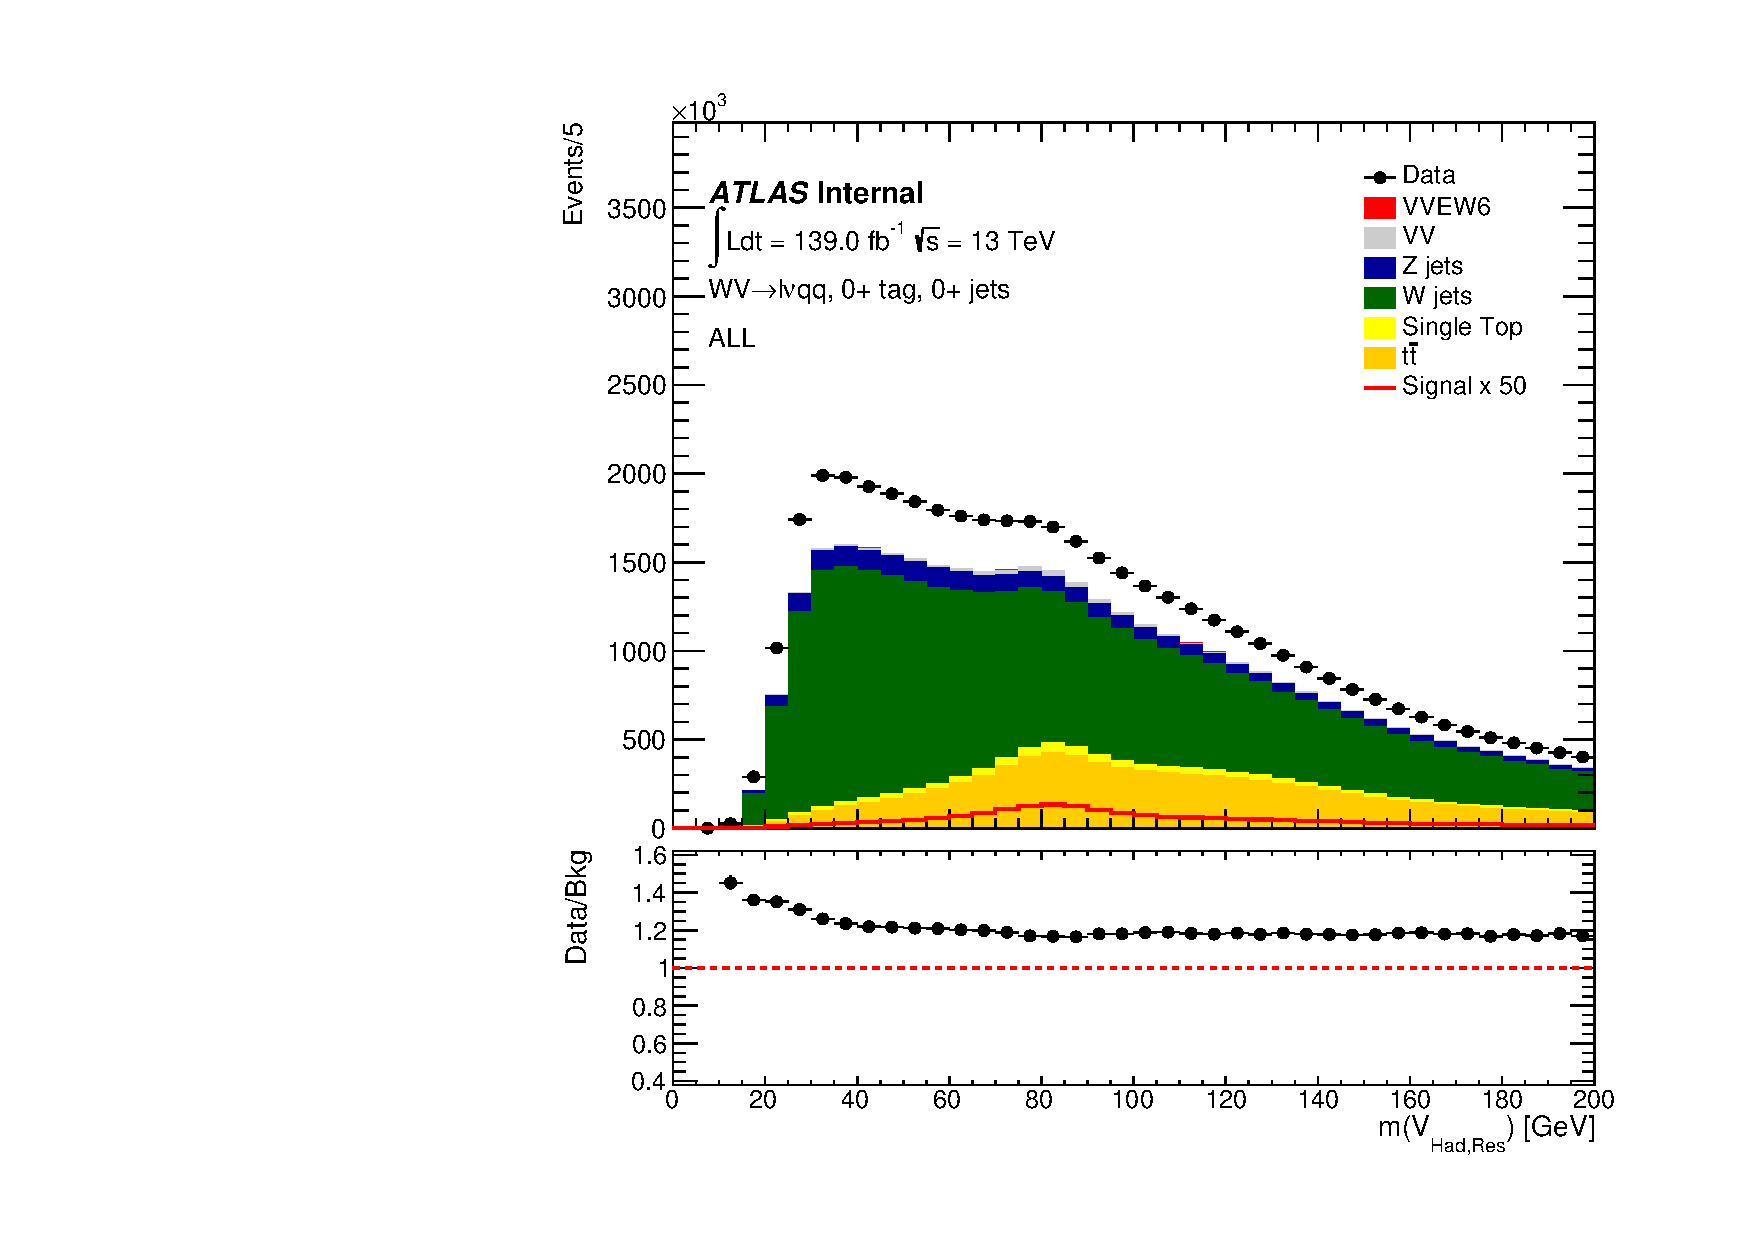
\includegraphics[width=\linewidth]{figures/event_selection/ALL_MVHadRes.pdf}
        \caption{Before any event selection.}
    \end{subfigure}
    \begin{subfigure}{0.32\textwidth}
        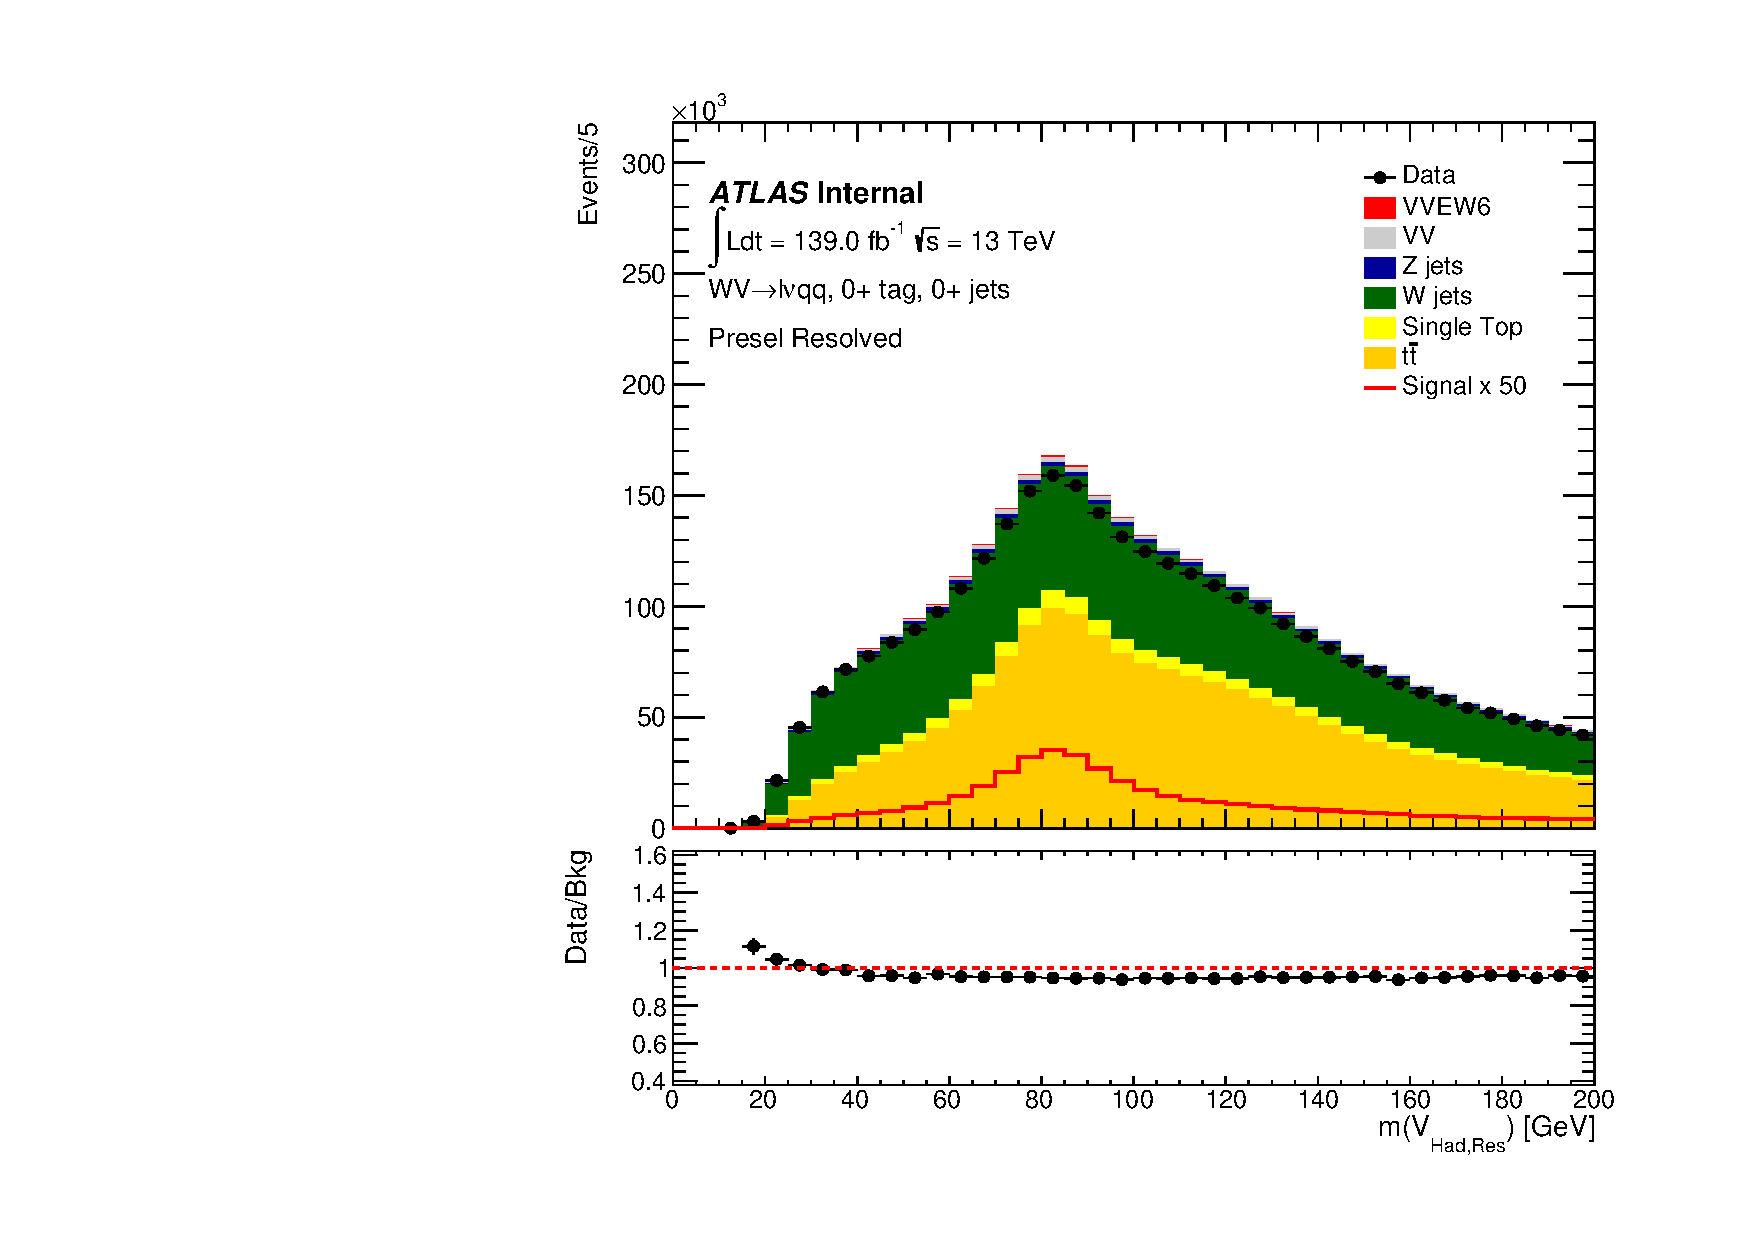
\includegraphics[width=\linewidth]{figures/event_selection/Presel_Resolved_MVHadRes.pdf}
        \caption{After resolved preselection.}
    \end{subfigure}
    \caption{Reconstructed mass distribution of the leading two jets.}
    \label{fig:1lepMVHadResSR}
\end{figure}

\subsection{VV system invariant mass}
\label{subsubsec:mVV_reconstruction}

The mass of the $WV$ system, $m_{WV}$, is calculated using the lepton, neutrino, and the hadronically-decaying boson (represented by either a large-$R$ jet or two small-$R$ jets). To determine the neutrino's momentum in the $z$-direction ($p_z$), we apply the Particle Data Group (PDG) value for the $W$ boson mass to the lepton-neutrino system. This results in a quadratic equation. The solution for $p_z$ is chosen based on the following criteria: if the solutions are complex, the real component is taken; if they are real, the solution with the smaller absolute value is selected.

%%%%%
